\documentclass[12pt, doublespace, oneside]{article}
\usepackage[utf8]{inputenc}
\usepackage{multirow}
\usepackage{physics}
\usepackage{float}
\usepackage{amsfonts}
\usepackage{graphicx}
\usepackage[english]{babel}
\usepackage{hyperref}
\usepackage{nicefrac}
\let\endtitlepage\relax
\usepackage[        
left=2cm,
right=2cm,
top=2.7cm,
bottom=2.7cm]{geometry}
    %\usepackage{showframe} %This line can be used to clearly show the new margins

% \newgeometry{hmargin={12mm,35mm}}  % set the margins
% \newgeometry{vmargin={25mm,25mm}}
\renewcommand{\baselinestretch}{1.3}

\title{{\vspace{-1.6cm}}East-West Method Analysis over the All Triggers Dataset}
\author{E.Coronel\footnote{evelyn.coronel@ib.edu.ar} ,  S. Mollerach}
\date{March 2021}

\begin{document}

\begin{titlepage}
\maketitle
\end{titlepage}


There are mainly two techniques are used in the study of large-scale anisotropies over the events rate measured by the Pierre Auger Observatory: Rayleigh and East-West methods. These methods are based on studying modulations over the cosmic rays flux $I_{\alpha, \delta}$ using harmonic functions, where $\alpha$ and $\delta$ stand for the right ascension and declination respectively. 

Given an energy range, the Rayleigh analysis uses the rate of events to estimate the amplitude and phase of an anisotropy between this range up to any order. Also, using the Rayleigh distribution, it is possible to obtain the probability of measuring the same amplitude magnitude as a fluctuation of an isotropic distribution of cosmic rays. This method has approximately a resolution of $\nicefrac{1}{n}$ cycles per year where $n$ is the period of the time to be analyzed \cite{resolucion_barrido}, therefore this method might be sensible to weather modulation in the signal measured by the Observatory or area variations over the surface detectors array. To use this method properly,  instrumental effects must be kept as low as possible because these effects induce spurious amplitudes in the analysis.


In the other hand, the East-West method consists of the harmonic function's approximation of the difference of rate of events measured by the Observatory arriving from the East and West directions recorded at a given sidereal time angle $\alpha^0$, i.e. the zenith's right ascension. The instrumental effects are removed for the analysis without any further corrections, but a downside of this method is its lower sensibility than the Rayleigh analysis \cite{taborda}.

\section{Rayleigh method}

Using a dipolar approximation, the Rayleigh method estimates the modulation over the CR flux $I(\alpha^0)$ in the following way:

\begin{enumerate}
    \item Given $N$ events to study, first we obtain the parameters $a$ and $b$:
    \begin{align}
        a = \frac{2}{N} \sum^N_{i=1}w_i\,\cos{\alpha_i} \qquad
        b = \frac{2}{N} \sum^N_{i=1}w_i\,\sin{\alpha_i} 
    \end{align}
    where $\alpha_i$  is the right ascension of the $i$ event and $w_i$ is the  weight of the exposure of the  event. The sum of all these weights is $\mathcal{N}=\sum^N_i w_i$.
    \item Then we compute the amplitude and phase of the first order approximation $r$ y $\phi$,
        \begin{align}
            r = \sqrt{a^2 + b^2} \qquad
            \phi_{EW} = \arctangent{\frac{b}{a} }
        \end{align}

      where  $r$ y $\phi$ are the amplitude and phase of the modulation of the first order's approximation.

      Using the Rayleigh distribution and a measured amplitude r,  it is possible to calculate the probability of obtaining the same amplitude due to an isotropic distribution of cosmic rays using the expression:
      \begin{equation}
        P({r}_k)= \exp(-\mathcal{N}\frac{{r}_k^2}{4})
      \end{equation}

      We can also use as a reference the value of an amplitude $r_{99}$, defined as $P(r_{99}) = 0.01\, (1\%)$:
      \begin{equation}
          r_{99} = \sqrt{-\log(0.01)\frac{4}{\mathcal{N}}}
      \end{equation}

      \item To generalize this analysis to any frequency, instead of using the right ascension $\alpha$, we used the variable:
      $\tilde{\alpha} = 2\pi f_x t_i $, where $f_x$ stands for the  frequency  of interest, and $t_i$ is the time in which the event was measured. It allows us to study the amplitude over solar frequency to verify the weather modulation over the SD signal.
      
\end{enumerate}

\section{East - West method}

Using a dipolar approximation, the East-West method estimates the modulation over the CR flux $I(\alpha^0)$ given by $I^{obs}_E -  I^{obs}_O$ in the following way:

\begin{enumerate}
    \item Given $N$ events to study, first we obtain the parameters $a_{EW}$ and $b_{EW}$:
    \begin{align}
        a_{EW} = \frac{2}{N} \sum^N_{i=1}\cos(\alpha^0_i - \beta_i) \qquad
        b_{EW} = \frac{2}{N} \sum^N_{i=1}\sin(\alpha^0_i - \beta_i)
    \end{align}
    where $\alpha^0_i$  is the Observatory's zenith right ascension at the moment of measurement of the $i$ event and $\beta_i=\pi$ if the event came from the East, $\beta=0$ otherwise.  
    \item Then we compute the amplitude and phase of the first orden approximation $r$ y $\phi$,
    
    \begin{tabular}{@{}p{.4\linewidth}@{}p{.5\linewidth}@{}}
        \begin{align}
            r_{EW} = \sqrt{a_{EW}^2 + b_{EW}^2} \\
            r   =\frac{\pi}{2} \frac{\langle\cos\delta \rangle}{\langle\sin\theta \rangle} r_{EW}\label{dperp} 
        \end{align}
        &    \begin{align}
            \phi_{EW} = \arctangent{\frac{b_{EW}}{a_{EW}}} \\
            \phi = \phi_{EW}+ \frac{\pi}{2} \label{phase_fisico}
        \end{align}
      \end{tabular}

      where the amplitude $r_{EW}$ and phase $\phi_{EW}$ are related to  $r$ y $\phi$, which are the amplitude and phase of the modulation of the first order's approximation. The values $\langle\cos\delta \rangle$ and $\langle\sin\theta \rangle$ are the mean value over all the events $i$. Althought Rayleigh and  East-West methods are slightly different, we can still calculate $P(r)$ and $r_{99}$  using modified expressions regarding $r_{EW}$.
      \begin{align}
        P(r) =  \exp(-\frac{N}{4}r_{EW}^2) \qquad
        r_{99} = \frac{\pi}{2} \frac{\langle\cos\delta \rangle}{\langle\sin\theta \rangle}\sqrt{-\log(0.01)\frac{4}{N}}
    \end{align}


      \item To generalize this analysis to any frequency, instead of using the variable $\alpha^0$ we used the variable:
      $\tilde{\alpha} = 2\pi f_x t_i $, where $f_x$ stands for the  frequency  of interest, and $t_i$ is the time in which the event was measured. It allows us to study the amplitude over frequencies used as references.

      \item Another variable used in this article is the component of the dipole amplitude $d_\perp$ in the equatorial plane. It can be calculated using the following expression:
      \begin{equation}
        d_{\perp} = \frac{\pi}{2\langle\sin\theta \rangle} r_{EW} \label{dperp} 
      \end{equation}
      
\end{enumerate}


In this article, we present the novel results over the All Triggers dataset. The results were calculated using the East-West method for different energy ranges and were compared with other published results obtained with the Herald dataset by the Collaboration.

\section{Datasets characteristics}

\paragraph{} The following events are classified by their energy, as they were reported by the Collaboration. These events are used to report and compare several results. The All Triggers dataset includes registered events from 2014 to 2020. Meanwhile, the Herald dataset contains data gathered from 2004 to 2018. The characteristics of both datasets are presented in Table \ref{tab:datasets}

\begin{table}[H]
    \vspace*{-1.5 cm}
    \begin{small}
        \begin{center}
            \begin{tabular}{lc|l|l|l|}
\hline
\multicolumn{1}{|l|}{\multirow{4}{*}{\begin{tabular}[c]{@{}c@{}}Time\\ span\end{tabular}}}    & All Triggers        & From  &\multicolumn{2}{l|}{January 1$^{st}$, 2014 } \\ \cline{3-5} 
\multicolumn{1}{|l|}{}                                                                            & 6 years             & To    &\multicolumn{2}{l|}{January 1$^{st}$, 2020} \\ \cline{2-5} 
\multicolumn{1}{|l|}{}                                                                            & Herald              & From  &\multicolumn{2}{l|}{January 1$^{st}$, 2004} \\ \cline{3-5}
\multicolumn{1}{|l|}{}                                                                            & 14.7 years          & To    &\multicolumn{2}{l|}{August 1$^{st}$, 2018} \\ \hline  \\

\hline                                                                          \multicolumn{2}{|c|}{Energy range [EeV]}                                                    & \multicolumn{1}{c|}{0.25 - 0.5}  & \multicolumn{1}{c|}{ 0.5  - 1 } &\multicolumn{1}{c|}{ 1 - 2 } \\ \hline
\multicolumn{1}{|l|}{\multirow{2}{*}{Events}}                            & All Triggers    & $3\,967\,368$     & $3\,638\,226$   & $1\,081\,846$ \\ \cline{2-5} 
\multicolumn{1}{|l|}{}                                                    & Herald & $770\,316$        & $2\,388\,467$   & $1\,243\,103$ \\ \hline
\multicolumn{1}{|l|}{\multirow{2}{*}{\begin{tabular}[c]{@{}c@{}}Mean \\ Energy\end{tabular}}} & All Triggers   & $0.38$           & $0.69$         & $1.32$       \\ \cline{2-5} 
\multicolumn{1}{|l|}{}                                                                             & Herald & $0.43$            & $0.70$          & $1.28$       \\ \hline
\end{tabular}
            \caption{Datasets characteristics for several energy ranges.}
            \label{tab:datasets}
        \end{center}
    \end{small}
    \vspace*{-1. cm}
\end{table}



\section{Results of the Fourier Analysis}
\subsection{Results in the 0.25 EeV - 0.5 EeV energy range}


In the table \ref{tab:primer_bin_data} are reported the results of this energy bin for the solar and sidereal frequency. These results are compared with reported values in the following paper \cite{Aab_2020}. All uncertainties are calculated using the probability density function described in \cite{linsley1975fluctuation}. The All Triggers uncertainties $\sigma_{x,y}$ are smaller than reported values since this dataset is $\sim 5$ times larger than the Herald dataset.




\begin{table}[H]
    \vspace*{-0.1 cm}
    \begin{small}
        \begin{center}
            \begin{tabular}[c]{l|c|c||c|}
\cline{2-4}                                        & \multicolumn{2}{c||}{All Triggers}    & \multicolumn{1}{c|}{Herald  }   \\ \hline
\multicolumn{1}{|l|}{Frequency:                  } & Solar	                & Sidereal	                & Sidereal \cite{Aab_2020}   \\ \hline
\multicolumn{1}{|l|}{Amplitude r [\%]:           } & $0.17^{+0.22}_{-0.07}$	& $0.12^{+0.24}_{-0.03}$ 	& $0.5^{+0.4}_{-0.2}$ \cite{codigo}      \\
\multicolumn{1}{|l|}{$r_{99}$ [\%]:             } & \multicolumn{2}{c||}{0.58}                          & 1.1\cite{codigo}                 \\
\multicolumn{1}{|l|}{$r^{UL}$ [\%]:             } & 0.67 	                & 0.64                      & 1.4\cite{codigo}                 \\ 
\multicolumn{1}{|l|}{$\sigma$[\%]:              } & \multicolumn{2}{c||}{0.19}                          & 0.38\cite{codigo}       \\\hline
\multicolumn{1}{|l|}{Amplitude $d_\perp$[\%]:    } & -	                    & $0.16^{+0.31}_{-0.04}$ 	& $0.6^{+0.5}_{-0.3}$       \\
\multicolumn{1}{|l|}{$d_{99}$ [\%]:             } & - 	                    & 0.73                      & 1.5  \cite{codigo}                \\
\multicolumn{1}{|l|}{$d_{\perp}^{UL}[\%]$       } & -                       & 0.80                      & 1.8                         \\
\multicolumn{1}{|l|}{$\sigma_{x,y}$[\%]:        } & -	                    & 0.24	                    & 0.48       \\\hline
\multicolumn{1}{|l|}{Probability      :        } & 0.66                    & 0.81	                    & 0.45       \\
\multicolumn{1}{|l|}{Phase [$^o$]:                } & 221$\pm$77              & 280$\pm$90                & 225$\pm$64\\ \hline
\multicolumn{1}{|l|}{$\langle\cos\delta \rangle$} & \multicolumn{2}{c||}{0.79}        	                & 0.79 \cite{codigo}        \\        
\multicolumn{1}{|l|}{$\langle\sin\theta \rangle$} & \multicolumn{2}{c||}{0.46}        	                & 0.52 \cite{codigo}        \\ \hline       
            \end{tabular}
            
        \end{center}
    \end{small}
    \vspace*{-0.5 cm}
    \caption{Obtained results in the All Triggers and Herald datasets for the solar and sidereal frequencies using the East method for the first harmonic approximation in the 0.25 EeV - 0.5 EeV energy bin. Some results were replicated using the code written for the paper Aab et a. 2020 \cite{Aab_2020}.}
    \label{tab:primer_bin_data}
\end{table}

The Fig. \ref{fig:primer} shows calculated phases on the All Triggers dataset using the East-West methods and compares these results with reported values of \cite{Aab_2020} on the Herald dataset. The dashed line indicates the direction of the galactic center, and the solid areas indicate de $1\sigma_{\phi}$ uncertainties of the phase using its probability density function  \cite{linsley1975fluctuation}. The previous table and this figure indicate that the uncertainty of the All Triggers dataset is wide in this energy bin,  due to the small $r$ amplitude compared to its $\sigma_{x,y}$.

\begin{figure}[H]
    \begin{small}
        \begin{center}
            \vspace*{-.5 cm}
            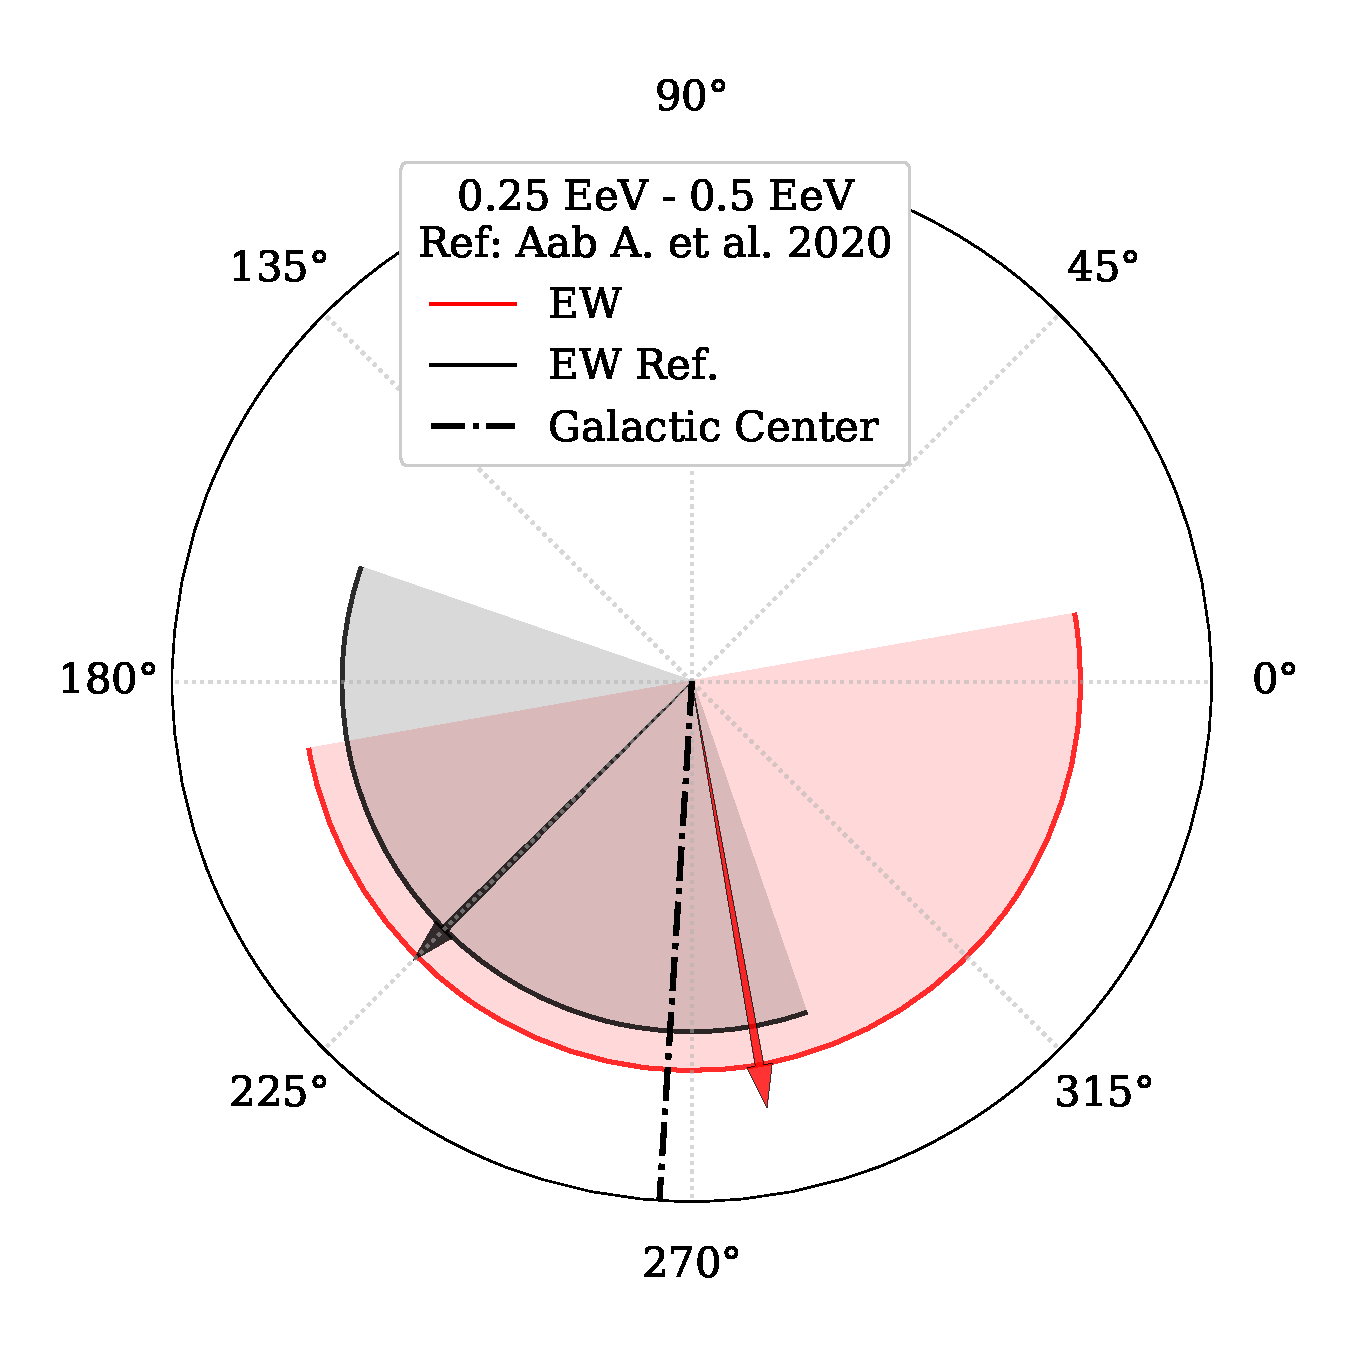
\includegraphics[width=0.65\textwidth]{Figs/phase_primer_bin_v3.pdf}
            \vspace*{-1 cm}
        \end{center}
        \caption{Phases values for the solar and sidereal frequencies in the 0.25 EeV - 0.5 EeV bin, as they were obtained for this article and reported by  Aab A. et al. (2020) \cite{Aab_2020} with their respective uncertainties. }
        \label{fig:primer}
    \end{small}
\end{figure}



Using the generalized variable $\tilde{\alpha}$, we obtain the Fig.\ref{fig:primer_barrido} that shows the amplitude for several frequencies, \ref{fig:primer_barrido}.  The dotted vertical lines represent, from left to right,  the anti-sidereal (364.25 cycles/year), solar (365.25 cycles/year), and sidereal (366.25 cycles/year). It is common to use these as references for this kind of analysis: instrumental and weather spurious amplitudes are present in these frequencies. Meanwhile, the amplitude calculated in the sidereal frequency is the first harmonic approximation for either Rayleigh or East-West methods. 


\begin{figure}[H]
    \begin{small}
        \begin{center}
            \vspace*{-1.2 cm}
            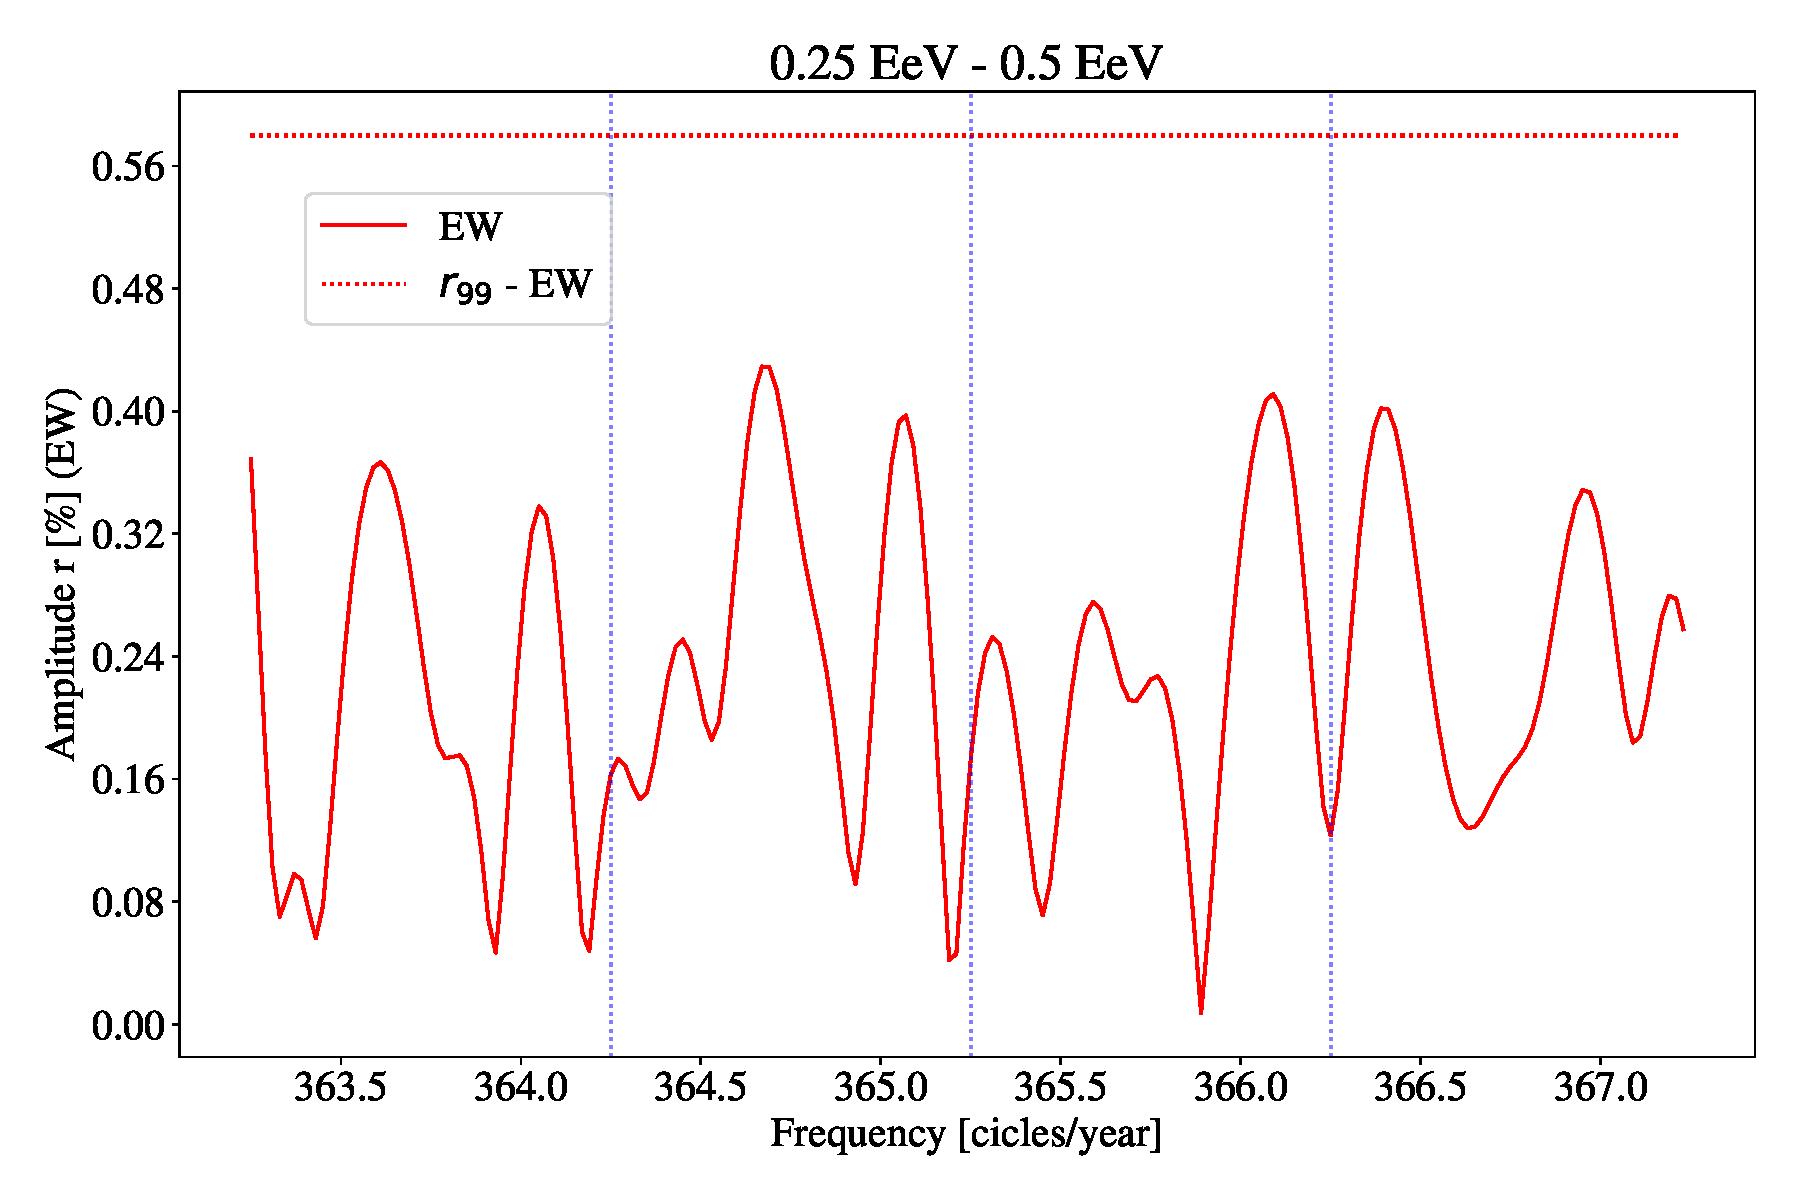
\includegraphics[width=0.8\textwidth]{Figs/plot_bin_1_barrido_v3_EW.pdf}
            \vspace*{-0.8 cm}
        \end{center}
        \caption{Fourier analysis of the modified variable $\tilde{\alpha}$ for events in the 0.25 EeV - 0.5 EeV bin from 2014 to 2020, using the East-West method on the All Triggers dataset. The dotted vertical lines represent, from left to right, the anti-sidereal, solar, and sidereal frequencies.}
        \label{fig:primer_barrido}
    \end{small}
\end{figure}

\subsection{Results in the 0.5 EeV - 1 EeV energy range}


In the table \ref{tab:segundo_bin_data} are reported the results of this energy bin for the solar and sidereal frequency. These results are compared with reported values in the following paper \cite{Aab_2020}. 




The Fourier analysis with the generalized variable $\tilde{\alpha}$ for this energy range is observed in Fig.\ref{fig:segundo_barrido}. The dotted horizontal line represents the $r_{99}$, none of the frequencies in the range showed in the previous figure exceeds the 1\% umbral. Also, this indicates that there are not spurious amplitudes in the anti-sidereal and solar frequencies.

In Fig. \ref{fig:segundo},  we compare the phases obtained in this article and the reference phase for this energy range in \cite{Aab_2020}. Their direction and uncertainty are similar. Also the galactic center is included in both uncertainties, indicated with a dashed line in the previous figure.

    \begin{table}[H]
        \vspace*{-0.8 cm}
        \begin{small}
            \begin{center}
                \begin{tabular}[c]{l|c|c||c|}
\cline{2-4}                                       & \multicolumn{2}{c||}{All Triggers}    & \multicolumn{1}{c|}{Herald  }   \\ \hline
\multicolumn{1}{|l|}{Frequency:                } & Solar	                & Sidereal	                 & Sidereal \cite{Aab_2020}   \\ \hline
\multicolumn{1}{|l|}{Amplitude r [\%]:           } & $0.43^{+0.21}_{-0.14}$	& $0.44^{+0.21}_{-0.14}$ 	& $0.38^{+0.20}_{-0.14}$ \cite{codigo}      \\
\multicolumn{1}{|l|}{$r_{99}$ [\%]:             } & \multicolumn{2}{c||}{0.56}                          & 0.64\cite{codigo}                 \\
\multicolumn{1}{|l|}{$r^{UL}$ [\%]:             } & 0.89 	                & 0.90                      & 0.90 \cite{codigo}                 \\ 
\multicolumn{1}{|l|}{$\sigma$[\%]:              } & \multicolumn{2}{c||}{0.18}                          & 0.21 \cite{codigo}      \\\hline
\multicolumn{1}{|l|}{Amplitude $d_\perp$[\%]:    } & -	                    & $0.56^{+0.27}_{-0.18}$ 	& $0.5^{+0.3}_{-0.2}$       \\
\multicolumn{1}{|l|}{$d_{99}$ [\%]:             } & - 	                    & 0.71                      & 0.8   \cite{codigo}                \\
\multicolumn{1}{|l|}{$d_{\perp}^{UL}[\%]$       } & -                       & 1.1                       & 1.1                         \\
\multicolumn{1}{|l|}{$\sigma_{x,y}$[\%]:        } & -	                    & 0.23	                    & 0.21       \\\hline
\multicolumn{1}{|l|}{Probability      :        } & 0.065                   & 0.055	                    & 0.20       \\
\multicolumn{1}{|l|}{Phase [$^o$]:                } & 205$\pm$34              & 258$\pm$34                & 261$\pm$43\\ \hline
\multicolumn{1}{|l|}{$\langle\cos\delta \rangle$} & \multicolumn{2}{c||}{0.79}        	                & 0.79 \cite{codigo}        \\        
\multicolumn{1}{|l|}{$\langle\sin\theta \rangle$} & \multicolumn{2}{c||}{0.50}        	                & 0.54\cite{codigo}        \\ \hline       
                \end{tabular}
            \end{center}
        \end{small}
        \vspace*{-0.4 cm}
        \caption{Obtained results in the All Triggers and Herald datasets for the solar and sidereal frequencies using the East method for the first harmonic approximation in the 0.5 EeV - 1.0 EeV energy bin. Some results were replicated using the code written for the paper Aab et a. 2020 \cite{Aab_2020}.}
        \label{tab:segundo_bin_data}
    \end{table}
    


    \begin{figure}[H]
        \begin{small}
            \begin{center}
                \vspace*{-0.9 cm}
                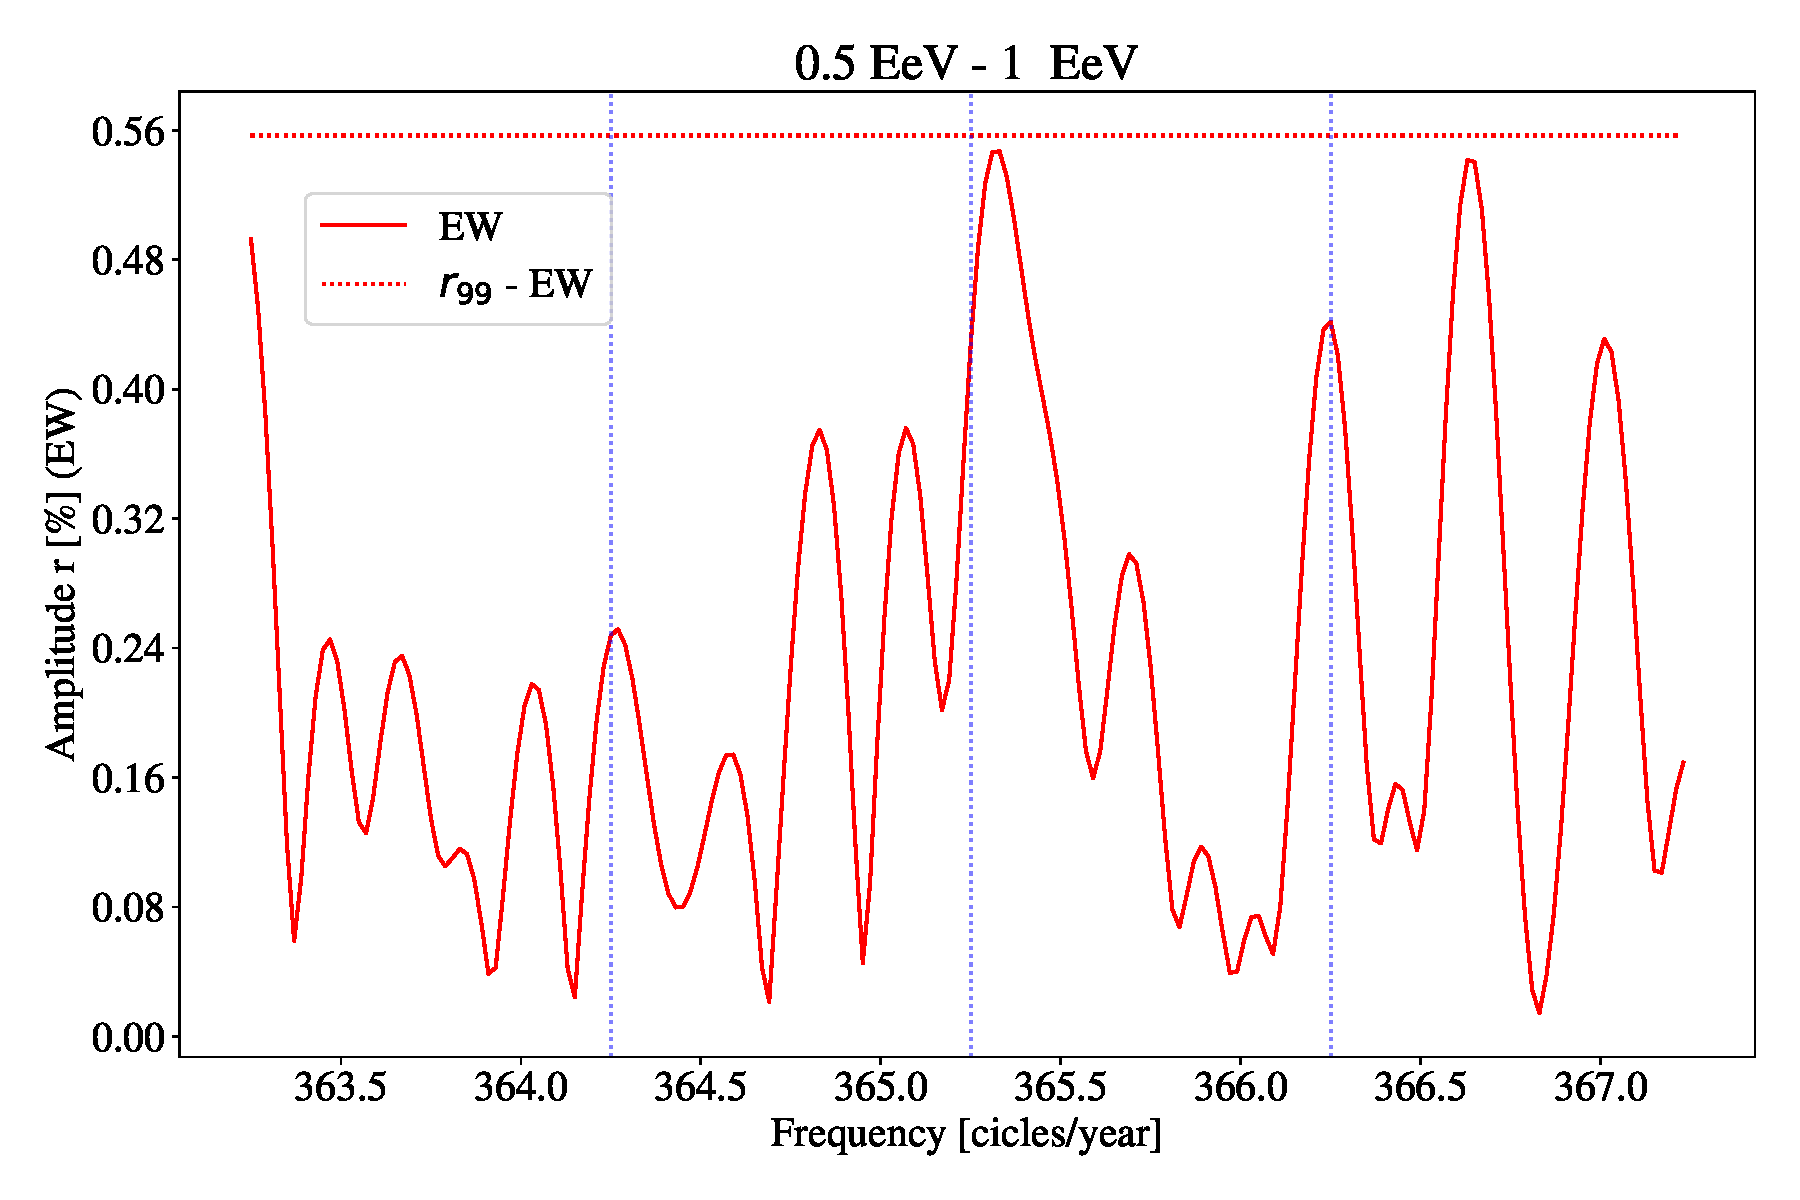
\includegraphics[width=0.8\textwidth]{Figs/plot_bin_2_barrido_v3_EW.pdf}
                
            \end{center}
            \vspace*{-1.1 cm}
            \caption{Fourier analysis of the modified variable $\tilde{\alpha}$ for events in the 0.5 EeV - 1.0 EeV bin from 2014 to 2020, using the East-West method on the All Triggers dataset. The dotted vertical lines represent, from left to right, the anti-sidereal, solar, and sidereal frequencies, whereas the horizontal line represents the limit of the 1\% of a amplitude produced by a isotropic flux of cosmic rays .}
            \label{fig:segundo_barrido}
        \end{small}
    \end{figure}    


    \begin{figure}[H]
        \begin{small}
            \begin{center}
                \vspace*{-0.65 cm}
                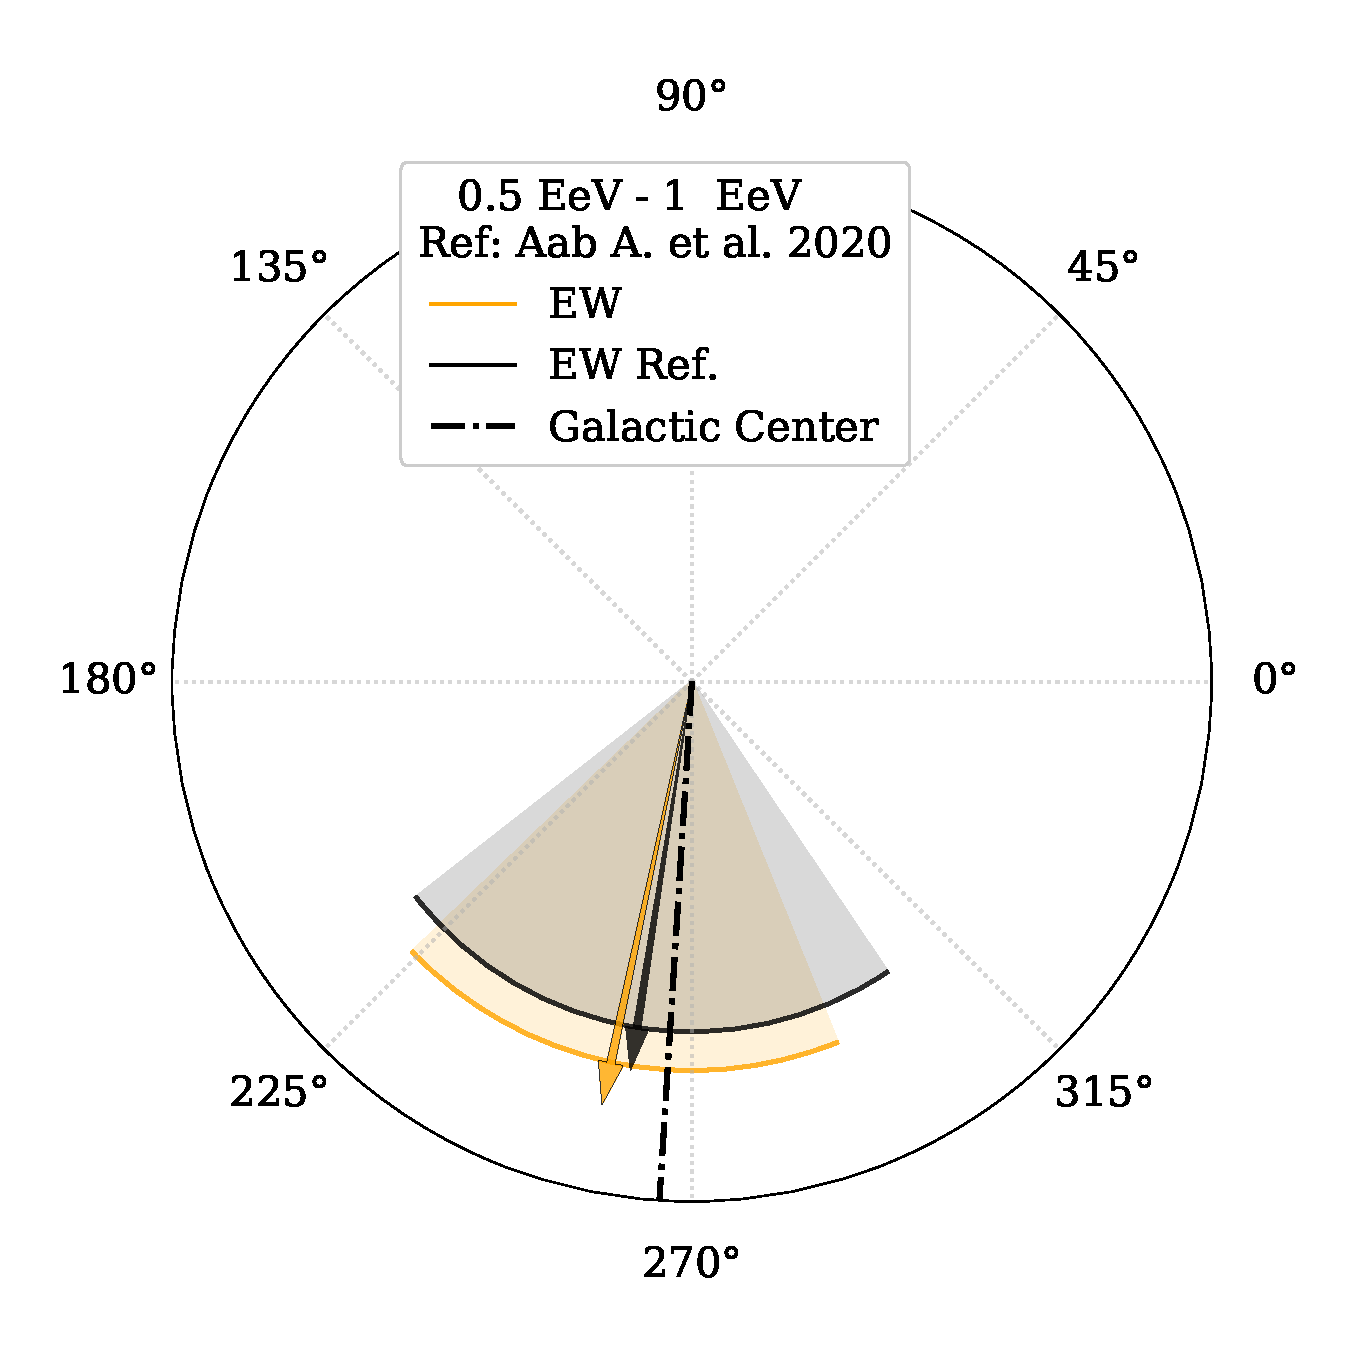
\includegraphics[width=0.65\textwidth]{Figs/phase_segundo_bin_v3.pdf}
                \vspace*{-1.1 cm}
            \end{center}
            \caption{Phases values for the solar and sidereal frequencies in the 0.5 EeV - 1 EeV bin, as they were obtained for this article and reported by  Aab A. et al. (2020) \cite{Aab_2020} with their respective uncertainties.}
            \label{fig:segundo}
        \end{small}
    \end{figure}


\subsection{Results in the 1.0 EeV - 2.0 EeV energy range}

For this energy range, it is possible to use both Rayleigh and East-West analysis, due to the All Triggers' full efficiency for lower energies. Therefore, we compare the results of these methods throughout this section.


In Table  \ref{tab:solar_3},  we compare the results of East-West and Rayleigh analysis for the solar frequency. The amplitudes are below the $r_{99}$ and are compatible between them. This indicates that weather modulation amplitudes in the solar frequency are low for All Triggers for either method.


\begin{table}[H]
    \vspace*{-0.81 cm}
    \begin{small}
        \begin{center}
            \begin{tabular}[c]{l|c|c|c|}
                \cline{2-4}         & \multicolumn{3}{c|}{All Triggers} \\ \cline{2-4}
                                    & Rayleigh   &                   & East - West            \\\hline
\multicolumn{1}{|l|}{Frequency:}       & \multicolumn{3}{c|}{Solar}        \\
\multicolumn{1}{|l|}{Amplitude $r$[\%]:} & $0.24^{+0.16}_{-0.09}$&         & $0.28^{+0.35}_{-0.11}$ \\
\multicolumn{1}{|l|}{$r_{99}$ [\%]:   } & 0.41                  &         & 0.91       \\
\multicolumn{1}{|l|}{$r_{UL}$ [\%]:   } & 0.58                  &        & 1.1       \\
\multicolumn{1}{|l|}{$\sigma$:        } & 0.14                  &         & 0.30          \\\hline
\multicolumn{1}{|l|}{Probability:    } & 0.22                  &          & 0.65          \\
\multicolumn{1}{|l|}{Phase  [$^o$] :           } & 260$\pm$48            &         & 279$\pm$76    \\\hline
            \end{tabular}
        \end{center}
        \vspace*{-0.41 cm}
    \end{small}
    \caption{Comparing results of the All Triggers dataset for the solar frequency using the East-West and Rayleigh method for the first harmonic approximation in the 1.0 EeV - 2.0 EeV energy bin. }
    \label{tab:solar_3}
\end{table}

Fig.\ref{tercer_barrido_Ray} shows the first harmonic amplitude of the Fourier analysis with the weighted Rayleigh method over the All Triggers dataset. The dotted vertical lines indicate the reference frequencies mentioned above, and the horizontal line is $r_{99}$. In this case, there are several amplitudes over the 1\% probability: one for the sidereal frequency and another one near the anti-sidereal frequency. The last peak shows a spurious amplitude and the presence of systematic error in the dataset.


\begin{figure}[H]
    \begin{small}
        \begin{center}
            \vspace*{-0.21 cm}
            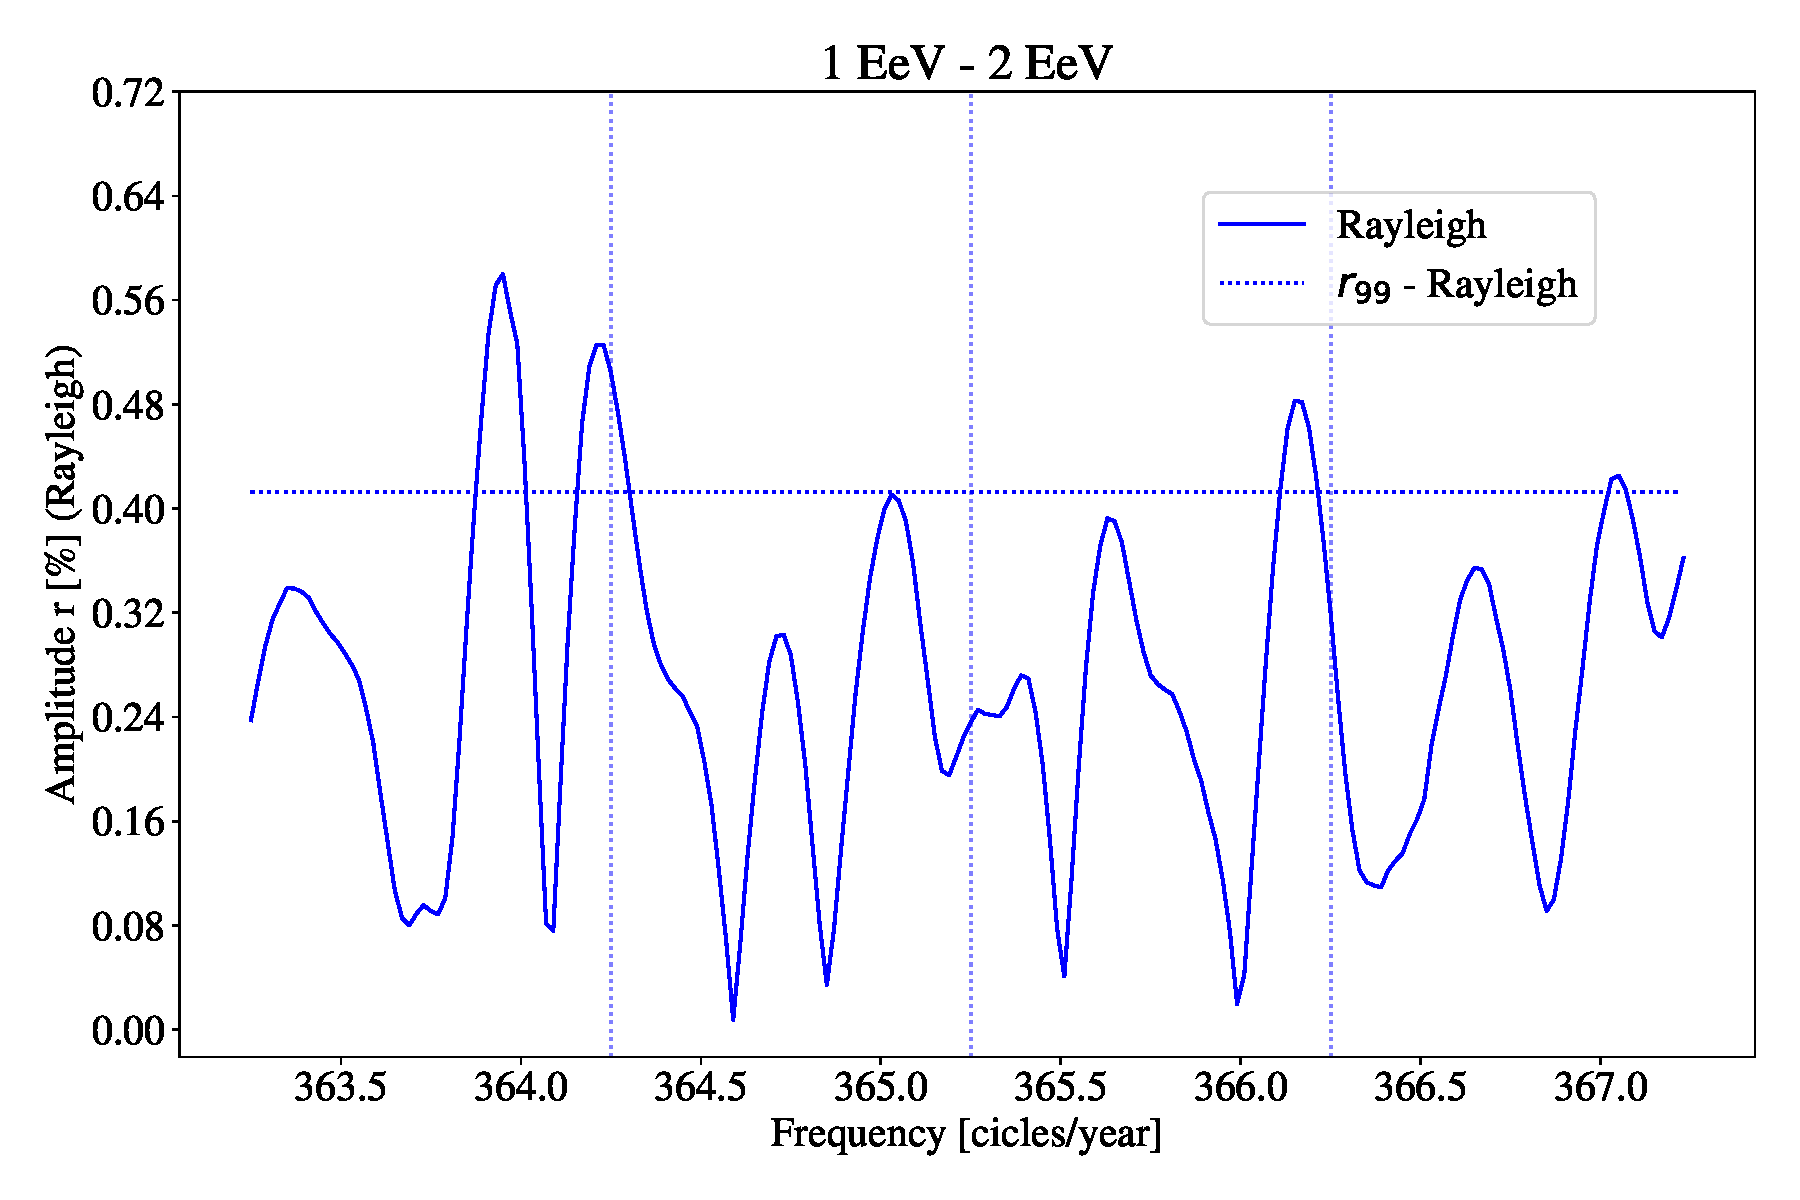
\includegraphics[width=0.9\textwidth]{Figs/plot_bin_3_barrido_v3_Ray.pdf}
            \vspace*{-1 cm}
        \end{center}
        \caption{Fourier analysis of the modified variable $\tilde{\alpha}$ for events in the 1.0 EeV - 2.0 EeV bin from 2014 to 2020, using the East-West method on the All Triggers dataset. The dotted vertical lines represent, from left to right, the anti-sidereal, solar, and sidereal frequencies, whereas the horizontal line represents the limit of the 1\% of a amplitude produced by a isotropic flux of cosmic rays .}
        \label{fig:tercer_barrido_Ray}
    \end{small}
\end{figure}    


Therefore, we need to use a method that is not as sensible as Rayleigh to systematic errors: the East-West analysis. The same Fourier analysis now using the East-West method is shown in Fig. \ref{fig:tercer_barrido}, now neither sidereal nor anti-sidereal frequencies show significant amplitudes. 


\begin{figure}[H]
    \begin{small}
        \begin{center}
            \vspace*{-0.21 cm}
            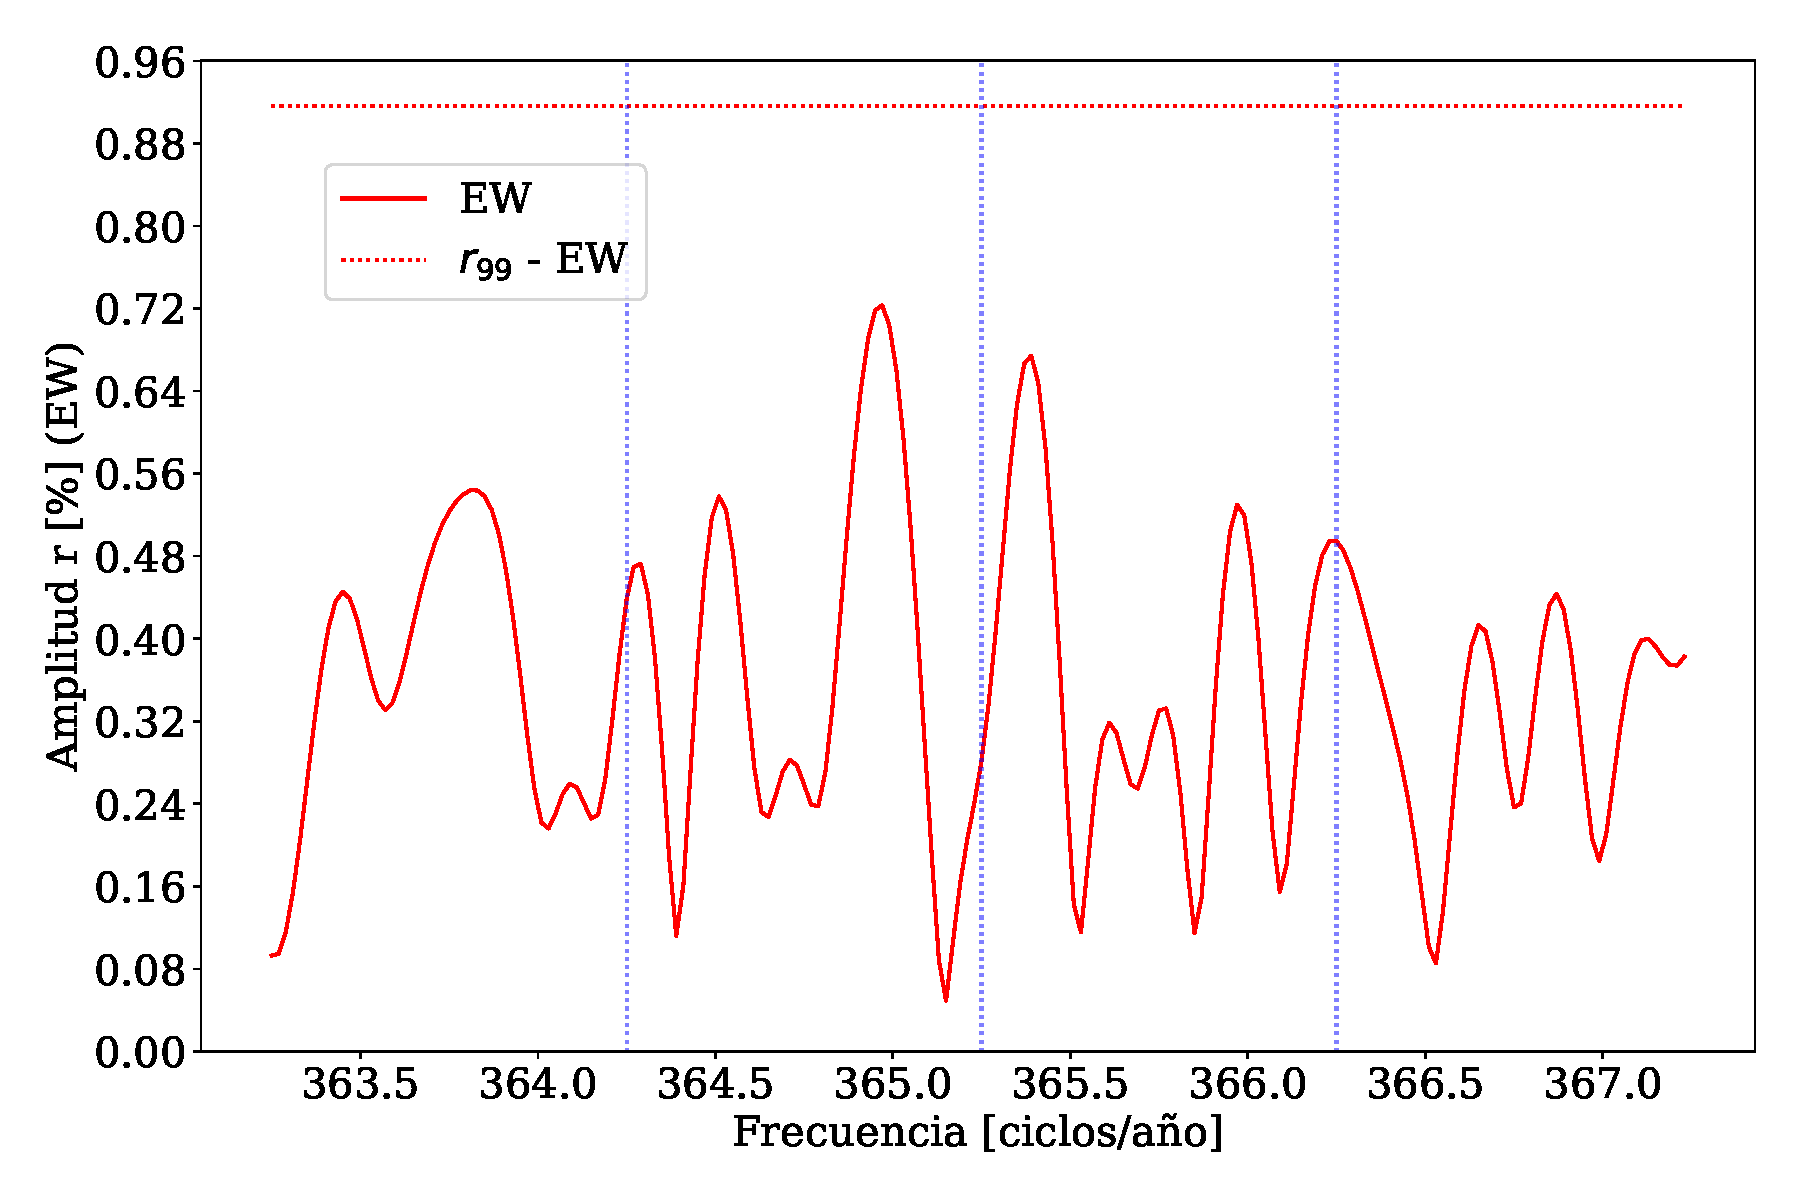
\includegraphics[width=0.9\textwidth]{Figs/plot_bin_3_barrido_v3_EW.pdf}
            \vspace*{-1 cm}
        \end{center}
        \caption{Fourier analysis of the modified variable $\tilde{\alpha}$ for events in the 1.0 EeV - 2.0 EeV bin from 2014 to 2020, using the Rayleigh method on the All Triggers dataset. The dotted vertical lines represent, from left to right, the anti-sidereal, solar, and sidereal frequencies.}
        \label{fig:tercer_barrido}
    \end{small}
\end{figure}    

More detailed results, for the sidereal frequency, can be found in Table  \ref{tab:siderea_3}: Rayleigh and East-West analysis for the All Triggers dataset, and reported values in \cite{Aab_2020} for the Herald dataset using the Rayleigh analysis.  



For the All Triggers dataset on the sidereal frequency, the amplitude calculated with the Rayleigh method has a probability of 6.3\%, meanwhile, the East-West method gives a 26\%. Knowing that this value depends on the number of analyzed events, this discrepancy cannot be attributed to different amounts of events: we are using the same dataset. 

    


    \begin{table}[H]
        \vspace*{-0.51 cm}
        \begin{small}
            \begin{center}
                \begin{tabular}[c]{l|c|c|c||c|}
                    \cline{2-5}                 & \multicolumn{3}{c||}{All Triggers}                  & Herald     \\
                    \cline{2-5}                 & Rayleigh               &       & East - West                 & East - West\cite{Aab_2020}      \\\hline
\multicolumn{1}{|l|}{Frequency:             }  & \multicolumn{3}{c||}{Sidereal}                               & Sidereal        \\ \hline
\multicolumn{1}{|l|}{Amplitude $r$ [\%]:      }  & $0.32^{+0.16}_{-0.10}$ &  	    & $0.5^{+0.3}_{-0.2}$         & $0.14^{+0.37}_{-0.02}$\cite{codigo}       \\
\multicolumn{1}{|l|}{$r_{99}$[\%]:           }  & 0.41	                 &         & 0.91                        & 0.84\cite{codigo}        \\
\multicolumn{1}{|l|}{$r^{UL}[\%]$      }        & 0.66                   &         & 1.3                         & 0.89 \cite{codigo}        \\
\multicolumn{1}{|l|}{$\sigma$[\%]:     }        & 0.14                   &         & 0.30	                    & 0.28 \cite{codigo}          \\ \hline
\multicolumn{1}{|l|}{Amplitude $d_\perp$ [\%]:}  & $0.41^{+0.20}_{-0.13}$ &         & $0.6^{+0.4}_{-0.3}$         & $0.18^{+0.47}_{-0.02}$       \\ 
\multicolumn{1}{|l|}{$d_{99}$[\%]:           }  & 0.53	                 &        & 1.1                         & 1.1\cite{codigo}        \\
\multicolumn{1}{|l|}{$d_{\perp}^{UL}[\%]$    }  & 0.84                   &         & 1.6                         & 1.1        \\
\multicolumn{1}{|l|}{$\sigma_{x,y}$[\%]:     }  & 0.17                   &         & 0.38	                    & 0.35          \\ \hline
\multicolumn{1}{|l|}{Probability:           }  & 0.063	                 &            & 0.26                        & 0.87          \\
\multicolumn{1}{|l|}{Phase [$^o$]:             }  & 357$\pm$35             &        & 320$\pm$48                 & 291$\pm$100      \\\hline
\multicolumn{1}{|l|}{$\langle\cos\delta\rangle$}&{0.78}&  &{0.78}                        & 0.78       \\        
\multicolumn{1}{|l|}{$\langle\sin\theta\rangle$}&{0.55}&  &{0.55}                        & 0.57       \\ \hline       
\end{tabular}
            \end{center}
        \end{small}
        \vspace*{-0.21 cm}
        \caption{Obtained results in the All Triggers and Herald datasets for the sidereal frequency using the East-West and Rayleigh method for the first harmonic approximation in the 1.0 EeV - 2.0 EeV energy bin. Some results were replicated using the code written for the paper Aab et a. 2020 \cite{Aab_2020}.}
        \label{tab:siderea_3}
    \end{table}

    
    A more visual way of comparing the phases between methods and datasets can be observed in Fig.\ref{fig:tercer}, where all results are compatible with $1\sigma$ uncertainty.


    \begin{figure}[H]
        \begin{small}
            \begin{center}
                \vspace*{-0.65 cm}
                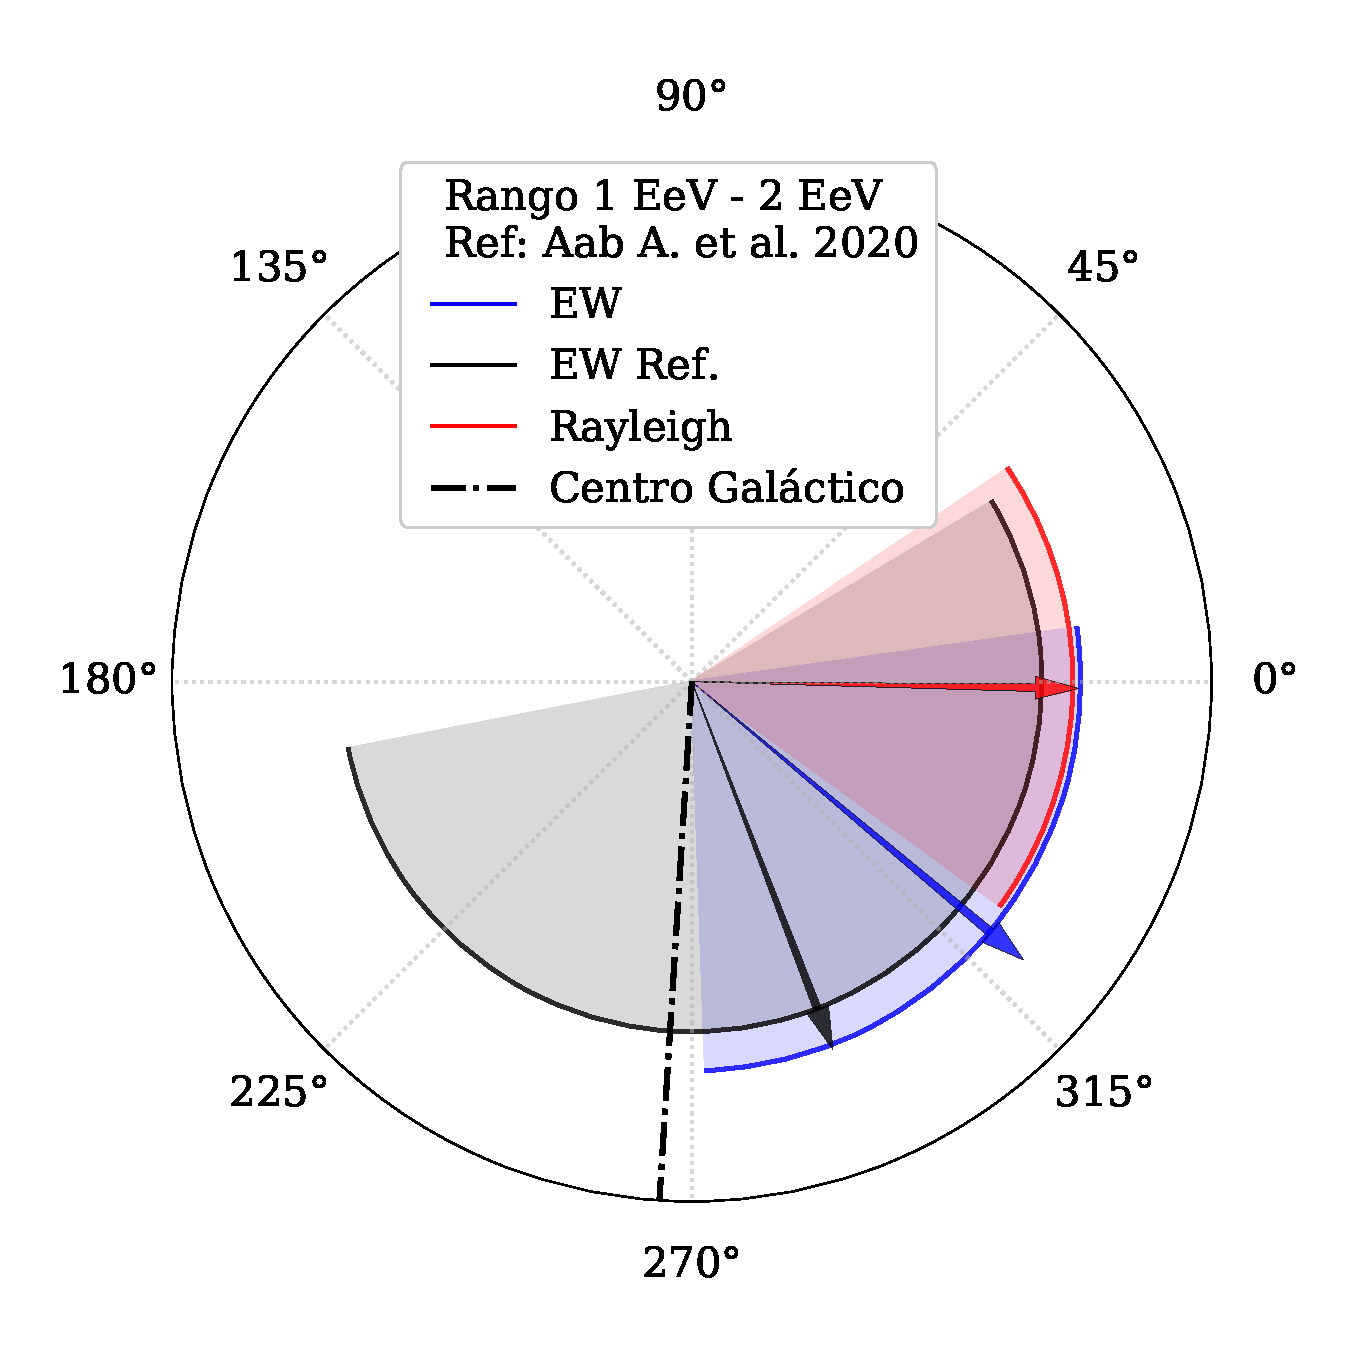
\includegraphics[width=0.65\textwidth]{Figs/phase_tercer_bin_v3.pdf}
                \vspace*{-1.2 cm}
            \end{center}
        \caption{Phases values for the solar and sidereal frequencies in the 1.0 EeV - 2.0 EeV bin, as they were obtained for this article and reported by  Aab A. et al. (2020) \cite{Aab_2020} with their respective uncertainties.}
        \label{fig:tercer}
        \end{small}
    \end{figure}

\section{Analysis}

    % El barrido de frecuencias para el conjunto de datos de All Triggers contiene datos de 6 años. Este rango de tiempo  permite tener una resolución de $\sim\nicefrac{1}{6}  \,$ciclos/año \cite{resolucion_barrido}. Los picos obtenidos en los barridos presentados en las Figs.\ref{fig:primer_barrido}, \ref{fig:segundo_barrido} y \ref{fig:tercer_barrido} están distanciados en promedio $\nicefrac{1}{5}\,$ciclos/año entre sí por lo que están dentro de la resolución posible del análisis. 

    % Una forma  para poder comparar los resultados de $d_\perp$ calculados de distintos conjuntos de  datos entre sí, es dividir estos valores con  sus respectivos $\sigma_{x,y}$. De esta manera, podemos comparar cuan apartados están con respecto $\sigma_{x,y}$. De esta manera se obtiene la Fig.\ref{fig:normalizado_sigma}, donde podemos decir que en los rangos entre 0.5 EeV - 1.0 EeV y 1.0 EeV - 2.0 EeV, la amplitude obtenida en este trabajo utilizando los eventos de All Triggers es más significativa que los resultados obtenidos por el trabajo \cite{Aab_2020} con el Herald  . Estos resultados difieren de trabajo \cite{Aab_2020} por $\sim 1\sigma_{x,y}$ y $\sim 2 \sigma_{x,y}$ respectivamente. Para comparar los resultados en el  rango 0.25 EeV - 0.5 EeV, tenemos que tener en cuenta que el Herald tiene una sensibilidad menor que el All Triggers. Esto se ve claramente en la Tabla \ref{tab:datasets}, donde el primero tiene 7 veces menos eventos para analizar que el segundo. Por lo tanto, la discrepancia entre este trabajo y los resultados presentados en \cite{Aab_2020} puede deberse a la  diferencia de eventos a estudiar causada por la sensibilidad del disparo.

    \begin{figure}[H]
        \begin{small}
            \begin{center}
                \vspace*{-0.21 cm}
                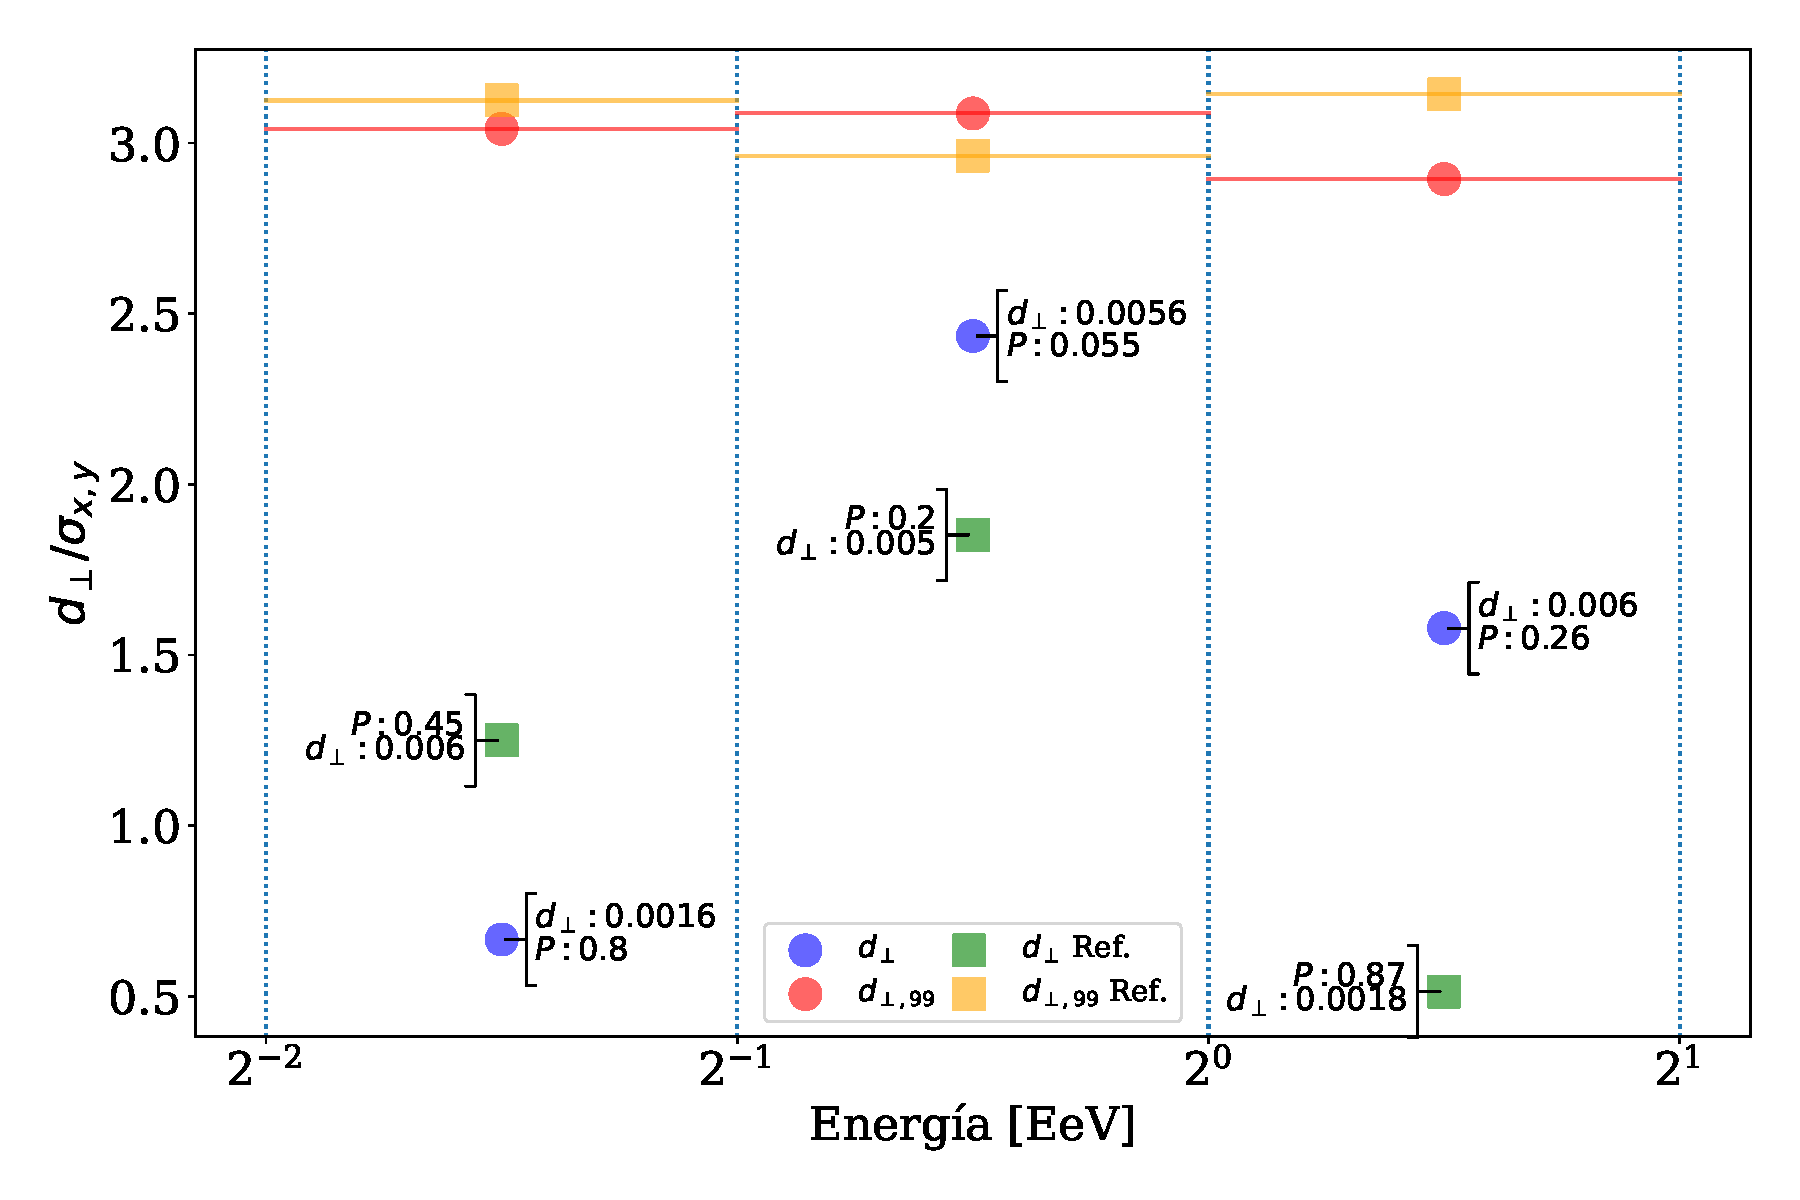
\includegraphics[width=\textwidth]{Figs/d_perp_normalizado_sigmas_v6.pdf}
                \vspace*{-1 cm}
            \end{center}
            \caption{Comparing amplitudes  $d_\perp$ and $d_{\perp,99}$  obtained with the East-West method over the All Triggers dataset in different energy bins. To compare these results, they are normalized with their respective uncertainties $\sigma_{x,y}$. }
            \label{fig:normalizado_sigma}
        \end{small}
    \end{figure}



    % Considerando los valores de $\sigma_{x,y}$ y $d_\perp$ obtenidos para cada rango de energía y con los métodos Rayleigh y East-West, es posible  comparar las direcciones, valores e incertidumbres en la Fig.\ref{fig:incertidumbre}. Las líneas punteadas están centradas en los valores reportados  en cada rango de energía por el trabajo \cite{Aab_2020}, obtenido con el Herald  . El  radio de cada círculo punteado igual al $\sigma_{x,y}$ de cada rango de energía. Los círculos sombreados indican el rango de incertidumbre  a $1\sigma_{x,y}$ de los valores obtenidos en este trabajo utilizando All Triggers. Cada flecha dentro de estos círculos sombreados indica a dirección y valor de $d_\perp$.    El punto asociado al método Rayleigh corregido con la modulación del clima de All Triggers en el rango 1-2 EeV se denota con \emph{Ray,mod}.

    % En los rangos de energía 0.25 EeV - 0.5 EeV y 0.5 EeV - 1.0 EeV, los valores obtenidos con All Triggers y el Heraldson compatibles entre sí dentro de la incertidumbre, además de contener la dirección al centro galáctico dentro de sus incertidumbres. Esto es interesante de resaltar ya que es esos rangos de energía, se espera que los rayos cósmicos sean galácticos.

    % En el rango 1.0 EeV - 2.0 EeV, se comparan resultados para el método de Rayleigh (\emph{Ray}) y el método East-West (\emph{EW}) obtenidos con All Triggers, y el valor obtenido por la Colaboración en el trabajo \cite{Aab_2020} mediante el  Rayleigh con el Herald  . Todos estos resultados son compatibles entre sí dentro de $1\sigma_{x,y}$ de incertidumbre. 

\begin{figure}[H]
    \begin{small}
        \begin{center}
            \vspace*{-0.21 cm}
            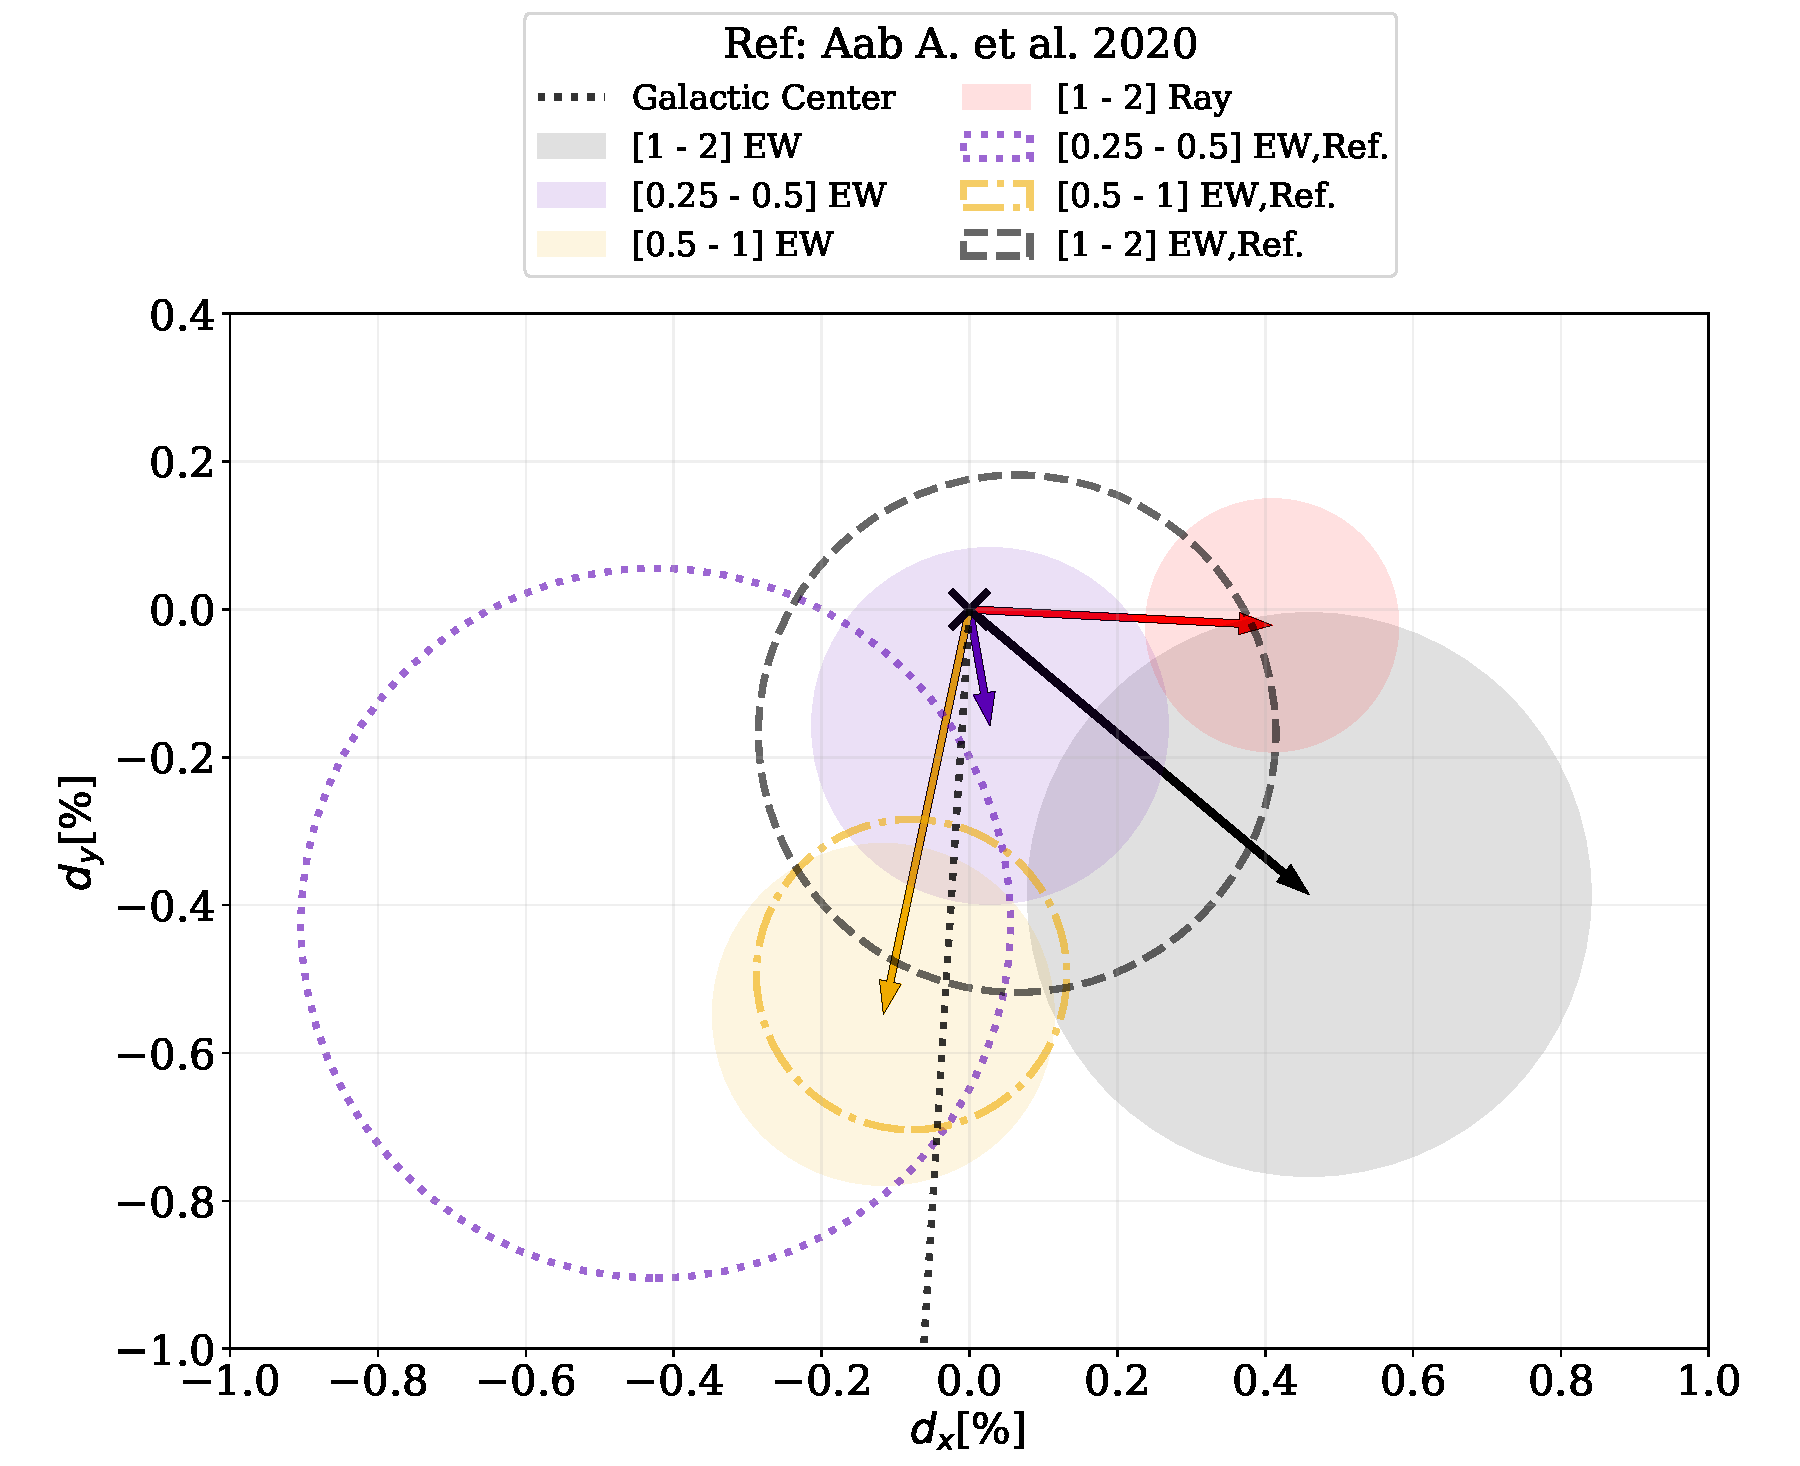
\includegraphics[width=\textwidth]{Figs/comparando_sigmas_v4.pdf}
            \vspace*{-1. cm}
        \end{center}
        \caption{Components of the dipole amplitude $d_\perp$ in the equatorial plane for several energy bins. The circles represent the $1\sigma_{x,y}$ uncertainties centered on the amplitudes and directions of each result. Dotted circles represent the values reported by \cite{Aab_2020} whereas solid circles denote the uncertainties calculated by this article. The dotted line indicates the direction of the galactic center.}
        \label{fig:incertidumbre}
    \end{small}
\end{figure}


\begin{thebibliography}{9}
    
  \bibitem{resolucion_barrido}
  Abreu, P., Aglietta, M., Ahn, E., Albuquerque, I., Allard, D., Allekotte, I.,
    \emph{et~al.}
   Search for first harmonic modulation in the right ascension
    distribution of cosmic rays detected at the Pierre Auger Observatory.
   \emph{Astroparticle Physics}, \textbf{34}~(8), 627 -- 639, 2011.
   \bibitem{taborda}
    Taborda, O. {Estudios de anisotropías a grandes escalas angulares de los rayos
  cósmicos de alta energía detectados por el Observatorio Pierre Auger}. PhD thesis, Instituto Balseiro, 2018. 
   
   \bibitem{Aab_2020}
    {Aab A. et al.},{Cosmic-Ray Anisotropies in Right Ascension Measured by the {Pierre   Auger Observatory}}.
    \emph{The Astrophysical Journal}, \textbf{891}~(2), 142, 2020. \url{https://doi.org/10.3847/1538-4357/ab7236}.
    \bibitem{linsley1975fluctuation}
    Linsley, J.
    Fluctuation effects on directional data.
     \emph{Physical Review Letters}, \textbf{34}~(24), 1530, 1975.

    
    \bibitem{codigo}  
    {Obtained using the code of the following paper \cite{Aab_2020}}.
\end{thebibliography}
    

\end{document}